\section{Task benchmark construction}
\label{sec:benchmark}
\subsection{Fixed task scope and reference answers}
Each question specifies a source tile, a geographic region of interest (ROI), an initial vehicle state, an answer vocabulary, and an annotation-derived reference answer. A building belongs to the reference ROI when its centroid lies inside the ROI bounds. Let $B_R$ be these buildings and $D_R\subseteq B_R$ the buildings labelled damaged. Minor, major, and destroyed xBD labels map to the binary damaged class; unclassified records do not define a binary answer. The reference answer is computed before a policy runs and is unchanged by later crops or movements.

The four task families capture different aspects of the trade-off between local detail and regional coverage. Presence asks whether $|D_R|>0$: a single convincing positive may suffice, whereas a negative answer requires evidence across the region. Damage asks for the binary state of a designated building, whose location is a permitted task cue. Count maps $|D_R|$ to $0$, $1$, $2$, or $3+$ and requires aggregation across the ROI. Spatial asks for the eight-sector bearing from the ROI center to the nearest damaged building and requires a nonempty $D_R$. Reference answers are derived from these annotation and geometry rules, independently of language-model generation.

Figure~\ref{fig:task-traces} illustrates how platform inputs are converted into task outputs. Spatial localization associates predicted damaged buildings with geographic position before computing a relative direction; damage counting aggregates building-level predictions over the visible region; and an active inspection instruction expands into navigation, descent, observation, and reporting actions. These platform-run examples illustrate the interface and are separate from the frozen 160-question evaluation set.

\begin{figure*}[!t]
\centering
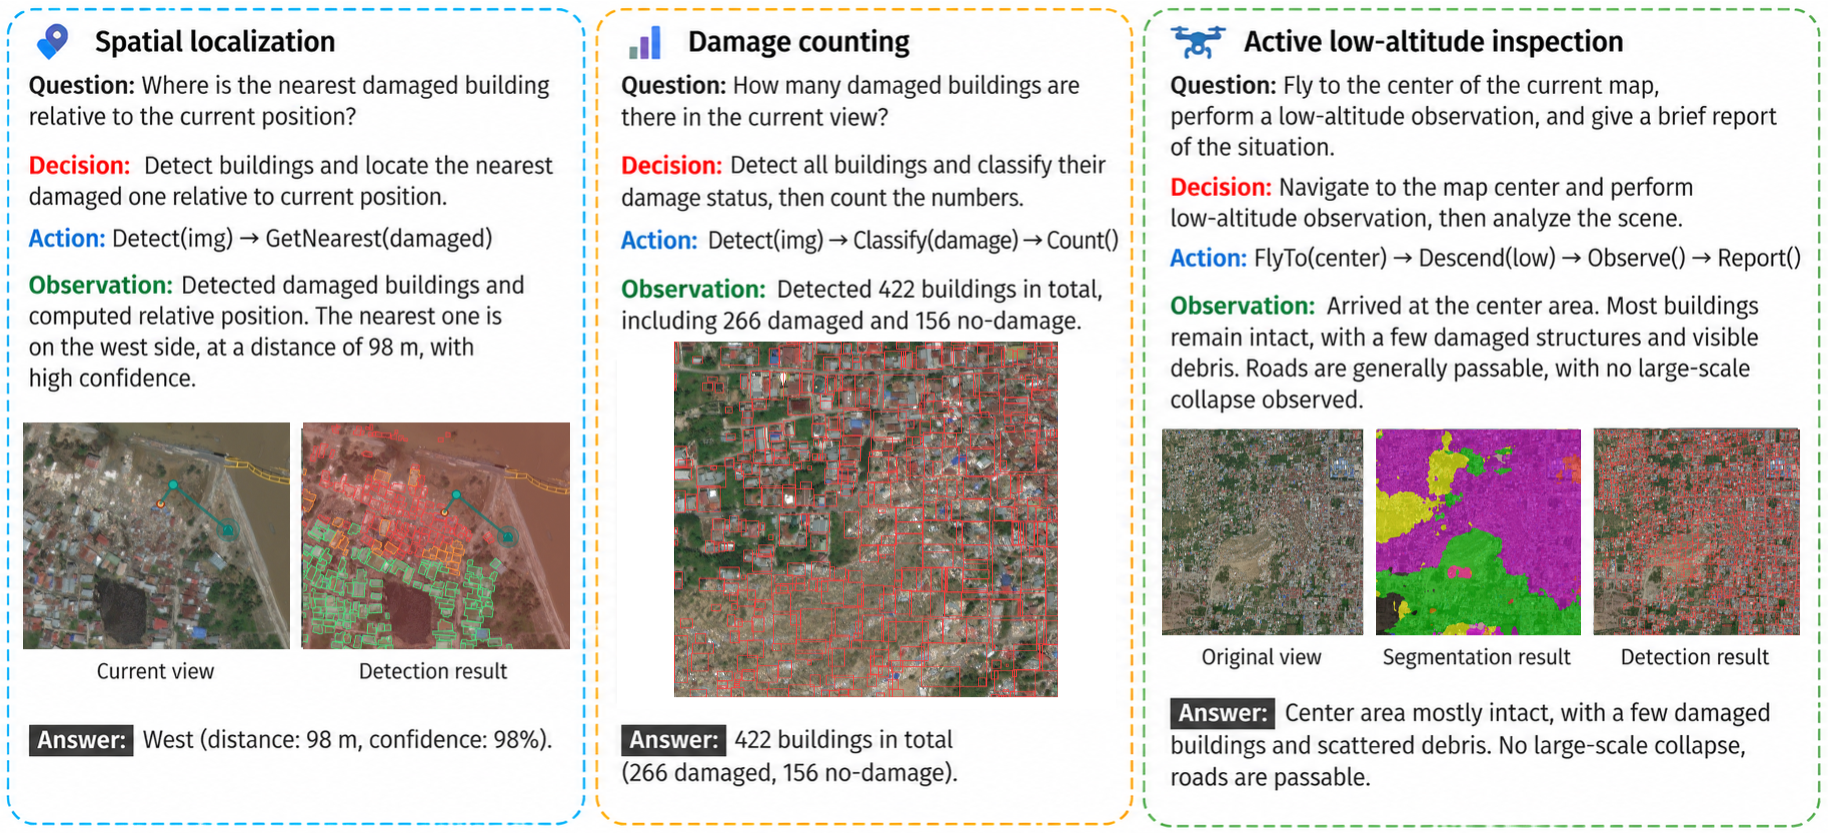
\includegraphics[width=\textwidth]{figure-paper/真正的输入输出.png}
\caption{Representative platform-run input--output traces. The examples show spatial localization from mapped detections, aggregation for damage counting, and an active low-altitude inspection sequence. They illustrate the interface and action vocabulary; quantitative results use the separately frozen benchmark and headless runner.}
\label{fig:task-traces}
\end{figure*}

\subsection{Final-set composition and input boundary}
The frozen set has 160 questions over 44 ROIs: 48 in Hurricane Michael, 51 in the Moore tornado, and 61 in Nepal flooding. Table~\ref{tab:answer-distribution} reports the answer counts. The count task is concentrated in $0$ and $3+$, with only one $1$ and no $2$; this class imbalance prevents count accuracy alone from establishing performance across all four categories. Spatial answers are more dispersed, but that task also requires finding the correct nearest damaged building. Questions from the same ROI share image context and therefore do not represent independent scenes.

\begin{table}[htbp]
\centering\small
\caption{Frozen question and answer distribution. Counts refer to distinct questions, before policy runs or generation repeats.}
\label{tab:answer-distribution}
\begin{tabularx}{\linewidth}{@{}l r X@{}}
\toprule
Task & $n$ & Reference answers (count)\\
\midrule
Presence & 44 & yes 30; no 14\\
Damage & 44 & damaged 29; no damage 15\\
Count & 43 & $0$: 14; $1$: 1; $2$: 0; $3+$: 28\\
Spatial & 29 & N 3; NE 4; E 3; SE 4; S 3; SW 3; W 4; NW 5\\
\bottomrule
\end{tabularx}
\end{table}

The source task record separates runtime inputs from scoring information. The controller receives the question, answer choices, ROI bounds, initial state, and a marked reference ID and coordinate only for a damage question. It receives detector-predicted boxes, probabilities, and geographic projections after observation. The reference answer, xBD damage labels and polygons, and the true nearest-damaged-building coordinate for a spatial question are restricted to benchmark construction and scoring. For spatial questions, the agent must select a target from predicted evidence because the ground-truth target coordinate is withheld.

Eligible records require usable post-disaster imagery, a geographic footprint, and building labels; pre-disaster imagery supplies the archival damage reference. The generator excludes consumed development tiles, checks answer vocabulary, geometry, duplicate records, and split membership, and retains ambiguity flags for review. The final questions underwent human review before the set was frozen. These checks document reference construction and the input boundary. Visual answerability and potential shortcuts require separate evaluation. Section~\ref{sec:results} therefore evaluates text-only and permitted-metadata controls on the same frozen set. The comparison assesses whether the complete image-aware pipeline outperforms controls using the permitted non-image inputs. Because the controls also use a modality-specific prompt and omit the hybrid rule path, the contrast does not isolate the causal effect of image access alone.
